\section{Data provenance and fixing synchronization}
\label{sec:data}

\subsection{Primary market and central bank sources}
Every series in this study comes directly from official exchange archives, public exchange APIs, or central-bank releases retrieved on November 13, 2026 with raw SHA-256 verification manifests stored alongside raw payloads. No simulated prices, synthetic interpolation, or multi-venue composite price substitutes enter the primary dataset. Table~\ref{tab:coverage} summarizes coverage and quality diagnostics across all instruments.

Bank Indonesia's official statistical downloads provide $1,415$ daily JISDOR business-day fixings from January 4, 2021 to November 12, 2026, with zero duplicate dates and zero missing values \citep{bi_sp233021,bi_padg072026}. On the domestic crypto side, direct queries to Indodax's TradingView historical endpoint return complete five-minute candles from January 1, 2021 to November 12, 2026 ($616,896$ bars per pair) for \texttt{BTCIDR}, \texttt{USDTIDR}, \texttt{ETHIDR}, \texttt{XRPIDR}, and \texttt{BTCUSDT}, plus $455,040$ one-minute bars across January--November 2026 for \texttt{BTCIDR} and \texttt{USDTIDR}. Zero-volume carry-forward bars constitute only $1.73\%$ of \texttt{BTCIDR} five-minute bars and $0.61\%$ of \texttt{USDTIDR} five-minute bars, versus $5.97\%$ for \texttt{ETHIDR}, $6.64\%$ for \texttt{XRPIDR}, and $78.57\%$ for \texttt{BTCUSDT}, which shows that domestic \texttt{BTC/USDT} lacks continuous depth compared with \texttt{BTC/IDR} and \texttt{USDT/IDR}.

Offshore benchmark prices come from Binance Spot monthly compressed kline archives with upstream SHA-256 checksums for \texttt{BTCUSDT}, \texttt{ETHUSDT}, and \texttt{XRPUSDT} across January 2021--November 2026 ($616,683$ raw five-minute bars, $0.005\%$ zero-volume rate). An inner join on UTC timestamps between Indodax ($616,896$ raw bars) and Binance ($616,683$ raw bars) produces $616,683$ regular five-minute paired observations ($605,150$ bars with positive volume on both Indodax \texttt{BTC/IDR} and \texttt{USDT/IDR}). Historical Binance \texttt{BTCBIDR} and \texttt{USDTBIDR} pairs run until their May 17, 2024 delisting ($354,645$ five-minute bars), while Binance's direct \texttt{BTCIDR} and \texttt{USDTIDR} pairs launch on November 29, 2025 ($100,362$ five-minute bars through November 12, 2026) \citep{binance_bidr_2024}. Live Tokocrypto kline APIs returned empty payloads, and Pintu/Reku public endpoints provide current snapshots without historical candle depth, so those venues are excluded. To measure the external USD/USDT peg wedge, Coinbase Exchange provides \texttt{USDT-USD} hourly ($n = 48,441$) and daily ($n = 2,020$) series back to its May 4, 2021 listing, paired with Kraken \texttt{USDTUSD} daily bars (Kraken's API returns $720$ completed daily bars plus the in-progress retrieval-day bar, or $721$ rows across November 23, 2024--November 13, 2026). Continuous indicative FX spot (\texttt{IDR=X}), ECB reference rates (Frankfurter API), and \texttt{EURUSD=X} placebo benchmarks supplement sensitivity and falsification analyses.

\begin{table}[htbp]
\centering
\caption{Data Provenance and Historical Coverage Summary (2021--2026)}
\label{tab:coverage}
\fontsize{6.3}{7.5}\selectfont\setlength{\tabcolsep}{2pt}
\begingroup
\begin{tabular}{@{}llccrr>{\raggedright\arraybackslash}p{3.4cm}@{}}
\toprule
Provider / Venue & Instrument & Freq. & Start--End (UTC) & Rows & Zero-Vol & Role / Limitations \\
\midrule
Bank Indonesia & JISDOR & 1d & 2021-01-04 to 2026-11-12 & 1,415 & -- & Official FX benchmark; bus. days \\
Indodax & BTCIDR & 5m & 2021-01-01 to 2026-11-12 & 616,896 & 1.73\% & Primary local BTC; 1.73\% stale \\
Indodax & USDTIDR & 5m & 2021-01-01 to 2026-11-12 & 616,896 & 0.61\% & Local stablecoin; 0.61\% stale \\
Indodax & ETHIDR & 5m & 2021-01-01 to 2026-11-12 & 616,896 & 5.97\% & Secondary ETH; 5.97\% stale \\
Indodax & XRPIDR & 5m & 2021-01-01 to 2026-11-12 & 616,896 & 6.64\% & Auxiliary XRP; 6.64\% stale \\
Indodax & BTCUSDT & 5m & 2021-01-01 to 2026-11-12 & 616,896 & 78.57\% & Route C venue; 78.57\% zero-vol \\
Binance Spot & BTCUSDT & 5m & 2021-01-01 to 2026-11-12 & 616,683 & -- & Global USDT ref.; SHA-256 \\
Binance Spot & ETHUSDT & 5m & 2021-01-01 to 2026-11-12 & 616,683 & -- & Global ETH ref.; SHA-256 \\
Binance Spot & XRPUSDT & 5m & 2021-01-01 to 2026-11-12 & 616,683 & -- & Global XRP ref.; SHA-256 \\
Binance Spot & BTCBIDR & 5m & 2021-01-01 to 2024-05-17 & 354,645 & -- & Delisted 2024-05-17 \\
Binance Spot & BTCIDR & 5m & 2025-11-29 to 2026-11-12 & 100,362 & -- & Launched 2025-11-29 \\
Coinbase & USDT-USD & 1h & 2021-05-04 to 2026-11-13 & 48,441 & -- & Listed 2021-05-04 (peg wedge) \\
Kraken & USDTUSD & 1d & 2024-11-23 to 2026-11-13 & 721 & -- & 720-bar API cap (validation) \\
\bottomrule
\end{tabular}\endgroup
\begin{minipage}{\textwidth}\footnotesize\vspace{3pt}
\emph{Notes:} All series retrieved directly from official endpoints or public historical archives with SHA-256 manifests. BI JISDOR excludes weekends and Indonesian holidays; Coinbase USDT-USD commenced trading May 4, 2021; Binance BIDR delisted May 17, 2024; Binance direct IDR pairs launched November 29, 2025.
\end{minipage}
\end{table}


\subsection{Timestamp synchronization protocol}
To avoid look-ahead bias and artificial timing premia, primary daily observations anchor each JISDOR business day $t$ at its four-regime configured UTC publication timestamp $\tau_t$: 03:00 UTC (10:00 WIB) through April 1, 2021 ($n = 62$ days); 08:15 UTC (15:15 WIB) from April 5, 2021 through May 31, 2022 ($n = 280$ matched days under pandemic operational hours); 09:15 UTC (16:15 WIB) from June 2, 2022 through March 31, 2026 ($n = 920$ days); and 08:15 UTC (15:15 WIB) from April 1, 2026 onward ($n = 152$ days under PADG No.\ 7/2026). Because both Binance Vision klines and Indodax TradingView candles timestamp each bar by its opening time while reporting the bar's closing price, we compute each candle's exact observation availability time as $\text{open\_time} + \Delta t$ ($\Delta t = 5\text{ minutes}$ for 5m bars; $1\text{ hour}$ for Coinbase \texttt{USDT-USD}). For each JISDOR date, we match backward to the most recent completed candle whose observation availability time is at or before $\tau_t$ (within a $300$-second tolerance for five-minute bars and $120$-minute tolerance for hourly Coinbase \texttt{USDT-USD}). This yields $n = 1,414$ synchronized business days across all three primary assets with zero look-ahead bias and $0.0\text{ s}$ matching lag relative to the configured schedule ($0.71\%$ stale zero-volume incidence on Indodax \texttt{BTC/IDR}, $3.75\%$ on \texttt{ETH/IDR}, and $3.39\%$ on \texttt{XRP/IDR}). One JISDOR release out of $1,415$ lacks a synchronous crypto bar within the $300$-second window at the sample boundary. Because Bank Indonesia does not archive ad-hoc pandemic or Ramadan operational-hour notices in machine-readable form, we verify in sensitivity checks that shifting all $280$ pandemic-regime days by $+60\text{ minutes}$ (to 09:15 UTC) or all $151$ June--December 2022 days by $-60\text{ minutes}$ (to 08:15 UTC) leaves mean $B_t^{crypto}$ within $[-0.92, -0.50]\text{ bps}$, the stablecoin--FX variance share within $[82.76\%, 84.09\%]$, and Johansen $\text{Trace}_{RA}$ within $[150.06, 150.50]$.

Figure~\ref{fig:coverage} displays raw coverage spans alongside regulatory milestones, and Figure~\ref{fig:prices} plots the resulting synchronized BTC/IDR, JISDOR-converted global BTC/USDT, and \texttt{USDT/IDR}--JISDOR series.

\begin{figure}[htbp]
  \centering
  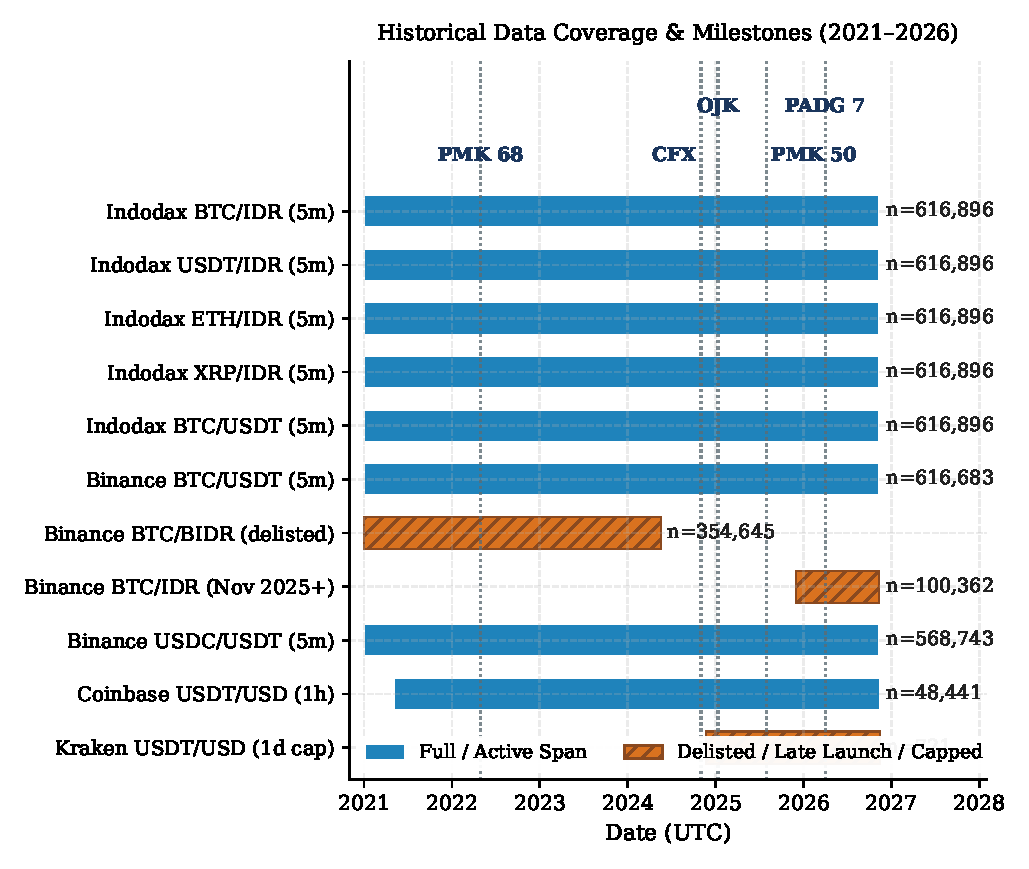
\includegraphics[width=\textwidth]{fig1_coverage_and_regimes.pdf}
  \caption{Historical instrument coverage matrix and Indonesian regulatory timeline (2021--2026).}
  \label{fig:coverage}
\end{figure}

\begin{figure}[htbp]
  \centering
  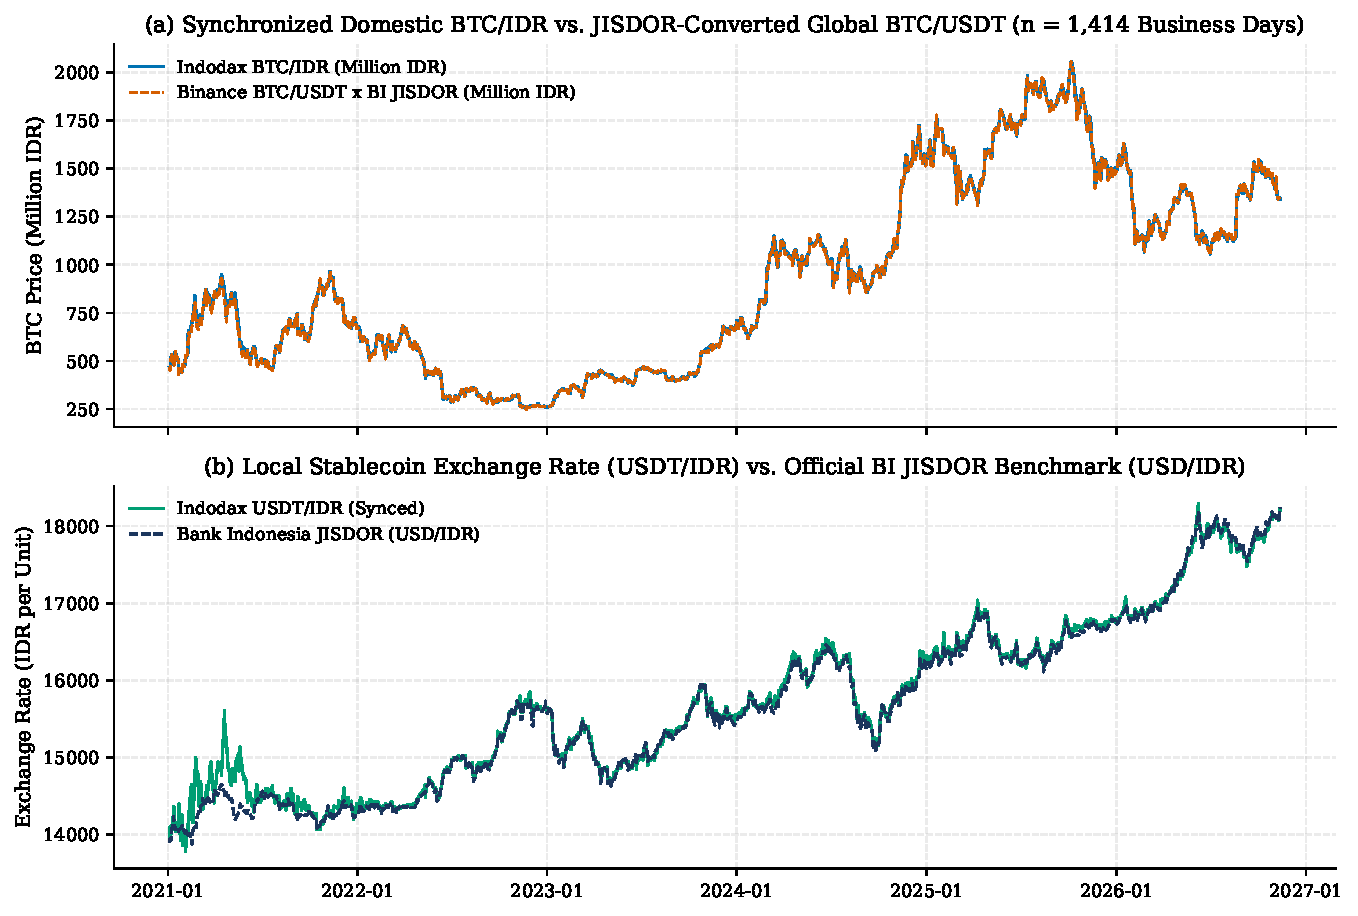
\includegraphics[width=\textwidth]{fig2_synchronized_prices.pdf}
  \caption{Synchronized domestic prices, JISDOR-converted global reference, and USDT/IDR vs.\ JISDOR (2021--2026).}
  \label{fig:prices}
\end{figure}
